\documentclass[oneside, openany]{memoir}
% hyperref must come first
\usepackage{hyperref}
\usepackage{amsfonts}
\usepackage[leqno]{amsmath}
\usepackage{amssymb}
\usepackage{amsthm}
\usepackage{colonequals}
\usepackage{enumitem}
\usepackage{mathabx}
\usepackage{mathtools}
\usepackage{thmtools}
\usepackage{tikz}
\usepackage{xspace}

\usepackage{tgpagella}
%\usepackage[sc]{mathpazo}
\usepackage{euler}
\usepackage{microtype}

\chapterstyle{companion}

\usetikzlibrary{arrows, matrix}

\addtolength\headheight{12pt}
\addtolength\parskip{.7ex}
\setlength\parindent{0cm}

\relpenalty=10000
\binoppenalty=10000

\setenumerate[1]{label = (\alph*), fullwidth}

\swapnumbers
\declaretheoremstyle[headfont = \scshape, bodyfont = \normalfont, qed = \qedsymbol]{foag}
\declaretheorem[style = foag, numberwithin = section]{exercise}
\renewcommand{\theexercise}{{\normalfont\textbf{\arabic{chapter}.\arabic{section}.\Alph{exercise}}}}

\newcommand\foreign[1]{\emph{#1}}
\newcommand\eg{\foreign{e.g.}}
\newcommand\Eg{\foreign{E.g.}}
\newcommand\ie{\foreign{i.e.}\xspace}
\newcommand\Ie{\foreign{I.e.}}
\newcommand\vs{\foreign{vs.~}}
\newcommand\cf{\foreign{cf.\xspace}}
\newcommand\resp{\foreign{resp.}}
\newcommand\etc{\foreign{etc.}}

\makeatletter
\newcommand*\map@arrow[1][]{\csname#1rightarrow\endcsname{}}
 
\newcommand*\function@textstyle[4][]{#2\colon#3\map@arrow[#1]#4}
\newcommand*\function[4][]{%
  \mathchoice
  {\function@textstyle[long#1]{#2}{#3}{#4}}
  {\function@textstyle[#1]{#2}{#3}{#4}}
  {\function@textstyle[#1]{#2}{#3}{#4}}
  {\function@textstyle[#1]{#2}{#3}{#4}}
}
\newcommand*\map@textstyle[6][]{#2\colon#3\rightarrow#4:#5\mapsto#6}
\newcommand*\map[6][]{%
  \mathchoice
    {#2\colon\
      \begin{array}{ccc}
        #3&~\map@arrow[long#1]~&#4 \\
        #5&~\longmapsto~&#6
      \end{array}
    }
  {\map@textstyle[#1]{#2}{#3}{#4}{#5}{#6}}
  {\map@textstyle[#1]{#2}{#3}{#4}{#5}{#6}}
  {\map@textstyle[#1]{#2}{#3}{#4}{#5}{#6}}
}
\makeatother

\newcommand\ball{\mathrm{B}}
\newcommand\category[1]{\mathsf{#1}}
\newcommand\dd{\;\!\mathrm{d}}
\newcommand\groupification{\mathrm{H}}
\newcommand\identity{\mathrm{id}}
\newcommand\projection{\pi}

\DeclareMathOperator\alg{alg}
\DeclareMathOperator\coker{coker}
\DeclareMathOperator\Hom{Hom}
\DeclareMathOperator\homology{H}
\DeclareMathOperator\image{im}
\DeclareMathOperator\Mor{Mor}
\DeclareMathOperator\pre{pre}
\DeclareMathOperator\res{res}
\DeclareMathOperator\sh{sh}
\DeclareMathOperator\SheafHom{\mathcal{H}om}
\DeclareMathOperator\Spec{Spec}
\DeclareMathOperator\Supp{Supp}

\title{Solutions to Foundations of Algebraic Geometry}
\author{Pieter Belmans}

\begin{document}

\maketitle

\begin{abstract}
  These notes contain my solutions to Ravi Vakil's Foundations of Algebraic Geometry. For more information I refer you to the official website/blog (\url{http://math216.wordpress.com/}) and the page with the actual notes (\url{http://math.stanford.edu/~vakil/216blog/}).
  
  The solutions are provided as is. I don't claim these to be correct or well written (although I certainly intend them to be for my own benefit). If you encounter any flagrant mistakes, you can contact me by e-mail (\url{pieterbelmans@gmail.com}) or add a patch to the GitHub repository at \url{https://github.com/pbelmans/math216}. Please do so by the way, preferably by submitting patches.

  As the notes are still being written when I started writing up these solutions and there may be changes to the numbering system upcoming: I am using the June 27 version. If I am still interested in these exercises when a final version is posted, I might edit in possible changes.
\end{abstract}

\clearpage

\tableofcontents*


\chapter{Introduction}
There are no exercises in this chapter.


\part{Preliminaries}

\chapter{Some category theory}
\section{Motivation}

There are no exercises in this section.


\section{Categories and functors}

\begin{exercise}
  \begin{enumerate}
    \item The elements of the group(oid) correspond to the category's morphisms. As every morphism is an isomorphism, we can only compose morphisms on the same object. Now in case of a single object, all axioms for a group are satisfied, as isomorphisms lead to inverse elements.

    \item Take the category of a group and copy the unique object, together with all its morphisms. Voil\`a, a groupoid.

      A natural example of groupoids is the fundamental groupoid of a topological space. You cannot combine loops that have different base points.
  \end{enumerate}
\end{exercise}

\begin{exercise}
  By definition of \emph{invertible element of~$\Mor(A,A)$} the automorphisms form a group: we get composition and associativity from the category and the identity and inverse from our choice of elements.
  
  In case of~$\category{Sets}$ the automorphisms are the permutations of the set, \ie, bijections. In case of~$\category{Vec}_k$ the automorphisms are bijective linear self-maps.

  By conjugation, isomorphic objects have isomorphic automorphism groups.
\end{exercise}

\begin{exercise} % TODO I should probably do this
  Linear algebra exercise. I will do this one if I feel inspired.
\end{exercise}

\begin{exercise}
  A basis for a finite-dimensional vectorspace has a well-defined cardinality, defining its dimension. So the inverse functor~$\category{f.d.\ Vec}_k\to\mathcal{V}$ maps an~$n$\nobreakdash-dimensional vectorspace~$V$ to~$k^n$, while every linear map between finite-dimensional vectorspaces can be written against a choice of bases. As we were allowed to pick a basis for each vectorspace simultaneously, every linear map admits by linear algebra magic with tons of indices a representation as a matrix.
\end{exercise}


\section{Universal properties determine an object up to unique isomorphism}

\begin{exercise}
  \label{exercise:23a}
  Take~$A$ and~$B$ initial objects. By definition of an initial object have (unique) morphisms~$A\to B$ and~$B\to A$, we can compose them, obtaining morphisms~$A\to A$ and~$B\to B$. But the identity is another candidate for this morphisms, so by uniqueness of the morphisms~$A$ and~$B$ are isomorphic.

  The proof for final objects is completely the same.
\end{exercise}

\begin{exercise}
  \begin{description}
    \item[$\category{Sets}$] The initial object is the empty set~$\emptyset$, the singleton~$\left\{ x \right\}$ is the final object (all singletons are isomorphic as stated before in~\autoref{exercise:23a}).
    \item[$\category{Rings}$] As the image of~$1\in\mathbb{Z}$ determines the entire ring morphism, the ring of integers~$\mathbb{Z}$ is the initial object. The final object is the trivial ring (in which~$0=1$).
    \item[$\category{Top}$] The initial object is the empty set~$\emptyset$ equipped with the topology consisting of~$1$~open set, the final object is the singleton equipped with the topology consisting of the empty set and the entire space.
  \end{description}

  The category subsets of a set and the category of open sets in a topological space are both \emph{bounded lattices}. Or, as there is either no morphism (if two sets are incomparable) or one morphism (if one set is contained in the other), we need to find objects that are either smaller or greater than all other objects. These are the empty set and the set~$X$.
\end{exercise}

\begin{exercise}
  Take~$s\in S$ a zerodisivor and let~$b\in A$ such that~$bs=0$. Now the image of~$b$ is equal to zero as
  \begin{equation}
    \frac{b}{1}=\frac{0}{1}\Longleftrightarrow s\left( b-0 \right)=0.
  \end{equation}

  Conversely, take~$a,b\in A$ and~$a\neq b$ such that their images are equal in the localization. That means there exists an~$s\in S$ such that~$s(a-b)=0$, so~$a-b\neq 0$ is a zerodivisor as~$0\notin S$.
\end{exercise}

\begin{exercise}
  \label{exercise:23d}
  The~$A$\nobreakdash-algebra~$S^{-1}A$ is a member of this category: an element of the multiplicative subset~$s\in S$ is a unit as it is inverted by~$1/s$. It is furthermore initial among these algebras because the unique morphism~$\overline{\varphi}\colon S^{-1}A\to B$ is given by~$\overline{\varphi}(r/s)=\varphi(r)\varphi(s)^{-1}$ where~$\varphi\colon A\to B$ is the structure map.

  Now this morphism~$\overline{\varphi}$ is unique because if~$\psi$ would be another morphism extending~$\mathrm{i}\colon A\to S^{-1}A$ we'd find
  \begin{equation}
    \psi\left( \frac{r}{s} \right)=\psi\left( \frac{r}{1} \right)\psi\left( \frac{1}{s} \right)=\varphi(r)\varphi(s)^{-1}
  \end{equation}
  as we split the fraction into parts on which~$\mathrm{i}$ works.
\end{exercise}

\begin{exercise}
  The definition of~$S^{-1}M$ is already given thoroughly in the hint, we obtain the map~$\phi\colon m\mapsto (m/1)$ because~$1\in S$ is required. The checks for the~$S^{-1}A$\nobreakdash-module structure are trivial and the universal property is satisfied by the proof from~\autoref{exercise:23d}.
\end{exercise}

\begin{exercise}
  The isomorphism is given by
  \begin{equation}
    \frac{1}{s}\left( m_1,\dots,m_n \right)\mapsto \left( \frac{m_1}{s},\frac{m_2}{s},\dots,\frac{m_n}{s} \right)
  \end{equation}
  with the inverse map being
  \begin{equation}
    \left( \frac{m_1}{s_1},\ldots,\frac{m_n}{s_n} \right)\mapsto\frac{1}{\prod_{i=1}^n s_i}\left( m_1\prod_{i\neq 1}s_i,\ldots,m_n\prod_{i\neq n}s_i \right).
  \end{equation}

  In the infinite case the product of the nominators is not defined. In the scenario of the hint that is given, the image under the inverse map has both a division by zero and a multiplication by infinity.
\end{exercise}

\begin{exercise}
  It is possible to proof that
  \begin{equation}
    \mathbb{Z}/(m)\otimes_\mathbb{Z}\mathbb{Z}/(n)\cong\mathbb{Z}/(d)
  \end{equation}
  with~$d\colonequals\gcd(m,n)$. In order to do so: observe that
  \begin{equation}
    x\otimes y=\left( xy \right)\otimes 1=xy\left( 1\otimes 1 \right)
  \end{equation}
  hence~$1\otimes 1$ is the generator of a cyclic group that represents the tensor product. Now~$d(1\otimes 1)=0$ because both~$m(1\otimes 1)$ and~$n(1\otimes 1)$ are zero by bringing it into the correct factor and using B\'ezout's identity. So the order of the cyclic group divides~$d$.
  
  Now we can map the direct product into~$\mathbb{Z}/(d)$ in an obvious way, which induces a map from the tensor product to~$\mathbb{Z}/(d)$. The element~$1\otimes 1$ is mapped to~$1$ and consequently has order~$d$, so there is an element of order \emph{at least~$d$}. Hence we have obtained the desired isomorphism.

  In this special case:~$\gcd(10,12)=2$, so~$\mathbb{Z}/(10)\otimes_{\mathbb{Z}}\mathbb{Z}/(12)\cong\mathbb{Z}/(2)$.
\end{exercise}

\begin{exercise}
  \label{exercise:23h}
  That~$f\otimes\identity\colon M\otimes N\to M''\otimes N$ is still surjective is obvious.

  For the surjection of~$M'\otimes N$ onto the kernel of~$f\otimes\identity$ we have to prove that in
  \begin{equation}
    M\otimes N\to (M\otimes N)/\image((M'\to M)\otimes\identity)\to M''\otimes N,
  \end{equation}
  the last morphism being the induced morphism from~$f\otimes\identity$ is invertible. Construct the induced~$\overline{\varphi}$ from
  \begin{equation}
    \map{\varphi}{M''\otimes N}{(M\otimes N)/\image((M'\to M)\otimes\identity)}{m''\otimes n}{m\otimes n+\image((M'\to M)\otimes\identity)}
  \end{equation}
  where~$m\in f^{-1}(m'')$ by surjectivity of~$f$. Now~$\varphi$ is well defined, bilinear and therefore extends to~$\overline{\varphi}$. Now the composition~$\overline{\varphi}\circ\overline{f\otimes\identity}$ is the identity, hence the induced morphism is invertible and we have obtained exactness.
\end{exercise}

\begin{exercise}
  Unique up to unique isomorphism means that the object is not necessarily unique, but all objects satisfying the universal property are isomorphic using a unique (iso)morphism (as~$f$ is said to be so). Hence these objects have trivial automorphism groups. By the same proof as for the universal property of categorical products this holds for tensor products.
\end{exercise}

\begin{exercise}
  The construction exactly quotients those objects that correspond to the bilinearity of the morphisms that are considered. Therefore all morphisms~$M\times N\to T'$ factor uniquely through~$T$.
\end{exercise}

\begin{exercise}
  \label{exercise:23k}
  \begin{enumerate}
    \item As stated in~\autoref{exercise:23d}: giving a ring map~$A\to B$ is the same as giving~$B$ an~$A$\nobreakdash-algebra structure. So we can consider both~$B$ and~$M$ as~$A$\nobreakdash-modules.

      We now use the fact that~$B$ is more than a module: it is an algebra. So we take by definition that~$B\otimes_A M$ interacts with scalars such that elements of~$B\setminus A$ are absorbed in the first factor, while scalar elements of~$A$ can (as by definition of the tensor product over~$A$) move around as we like.
      
      Let's tediously check all module axioms now. Take~$b_1,b_2\in B$ as scalars for the~$B$\nobreakdash-structure and~$b\otimes m,b'\otimes m'\in B\otimes_A M$ as $B$\nobreakdash-module elements. We have
      \begin{description}
        \item[$r(x+y)=rx+ry$:] This one is immediate.

        \item[$(r+s)x=rx+sx$:] We manipulate:
          \begin{equation}
            \begin{aligned}
              (b_1+b_2)(b\otimes m)&=(b_1+b_2)b\otimes m \\
              &=(b_1b+b_2b)\otimes m \\
              &=b_1b\otimes m+b_2b\otimes m \\
              &=b_1(b\otimes m)+b_2(b\otimes m)
            \end{aligned}.
          \end{equation}

        \item[$(rs)x=r(sx)$:] By definition of the~$B$\nobreakdash-module structure we obtain
          \begin{equation}
            (b_1b_2)(b\otimes m)=b_1b_2b\otimes m=b_1(b_2b\otimes m).
          \end{equation}

        \item[$1_Rx=x$:] We easily obtain
          \begin{equation}
            1_B(b\otimes m)=1_Bb\otimes m=b\otimes m.
          \end{equation}
      \end{description}

      The~$A$\nobreakdash-linearity (we're taking the tensor product over~$A$) is induced by the construction and requires no explicit checking.

      The functorality of the mapping~$\category{Mod}_A\to\category{Mod}_B$ follows from assigning to each morphism~$f\colon M_1\to M_2$ in the first category the map~$\identity\otimes f$ in the second.

    \item Now both~$B$ and~$C$ carry the desired~$A$\nobreakdash-algebra structure necessary for this multiplication to hold and the result follows from the previous point.
  \end{enumerate}
\end{exercise}

\begin{exercise}
  The natural isomorphism is given by
  \begin{equation}
    \frac{a}{s}\otimes m\mapsto \frac{am}{s}
  \end{equation}
  which is compatible with both the~$S^{-1}A$- and~$A$\nobreakdash-module structure by definition of~$S^{-1}M$. The inverse map is obviously defined as
  \begin{equation}
    \frac{m}{s}\mapsto \frac{1}{s}\otimes m
  \end{equation}
  and this is the correct inverse because we're tensoring over the ring~$A$.
\end{exercise}

\begin{exercise}
  The condition imposed on the elements of the Cartesian product that will act as the fibered product in~$\category{Sets}$ are necessary by the commutativity of the square. The maps~$\projection_X$ and~$\projection_Y$ are the obvious projections on the first or second factor.

  A map~$W\to X\times_Z Y$ is by the agreement of compositions to~$W$ given by using the maps~$W\to X$ and~$W\to Y$ for each component. Now this must be unique: if we'd try to fit in another map the commutativity of the diagram is broken.
\end{exercise}

\begin{exercise}
  It is the \emph{intersection} of the open sets: the fibered product must be an element of the category (which in this case only contains open sets). As for morphisms: these depict inclusion ($U\subseteq V$ implies $U\to V$) and are either unique or non-existing. So if~$W$ is a map to both~$X$ and~$Y$ which map to~$Z$, we have a chain of inclusions in which we can fit~$W\subseteq X\cap Y$.
\end{exercise}

\begin{exercise}
  The definition of fibered product depends on the choice of~$f$ and~$g$. But as~$Z$ is the final object, these morphisms are unique. Now place the product in the position reserved for the fibered product in the definition. As the compositions from~$W$ to~$Z$ agree ($Z$ being final implies uniqueness of these maps, hence equality!) we have a unique isomorphism between these two products.
\end{exercise}

\begin{exercise}
  The projection~$U\to V$ is given by the definition of the fibered product in the second square. The projection~$U\to Y$ is given by composing the projections~$U\to W$ and~$W\to Y$. The compositions of the obtained projections with both~$V\to Z$ and~$X\to Z$ agree by commutativity of the diagram.

  Now take an object~$A$ with maps~$A\to V$ and~$A\to Y$ such that the compositions with~$V\to Z$ and~$Y\to Z$ agree. We wish to consider a unique map~$A\to U$. Consider the map~$A\to W$ (which exists by chasing the diagram), by definition of the first fibered product, this map is unique.
  
  Now consider~$A\to V$, we have defined~$V\to Z$ by the composition of projections. By commutativity of the diagram~$A\to W\to X$ and~$A\to V\to X$ agree so we can use the second fibered product. So just construct a unique map~$A\to U$. We have obtained a tower of fibered products.

  Essentially, it boils down to lifting~$A\to Y$ to~$A\to W$ in a unique way.
\end{exercise}

\begin{exercise}
  Let's draw a picture.
  \begin{equation}
    \begin{tikzpicture}[description/.style = {fill = white, inner sep = 2pt}, baseline=(current bounding  box.center)]
      \matrix (m) [matrix of math nodes, row sep = 3em, column sep = 3em, text height = 1.5ex, text depth = 0.25ex]
      {
        X_1\times_Y X_2 & X_2 & X_2 \\
        X_1 & Y & \\
        X_1 & & Z \\
      };
      \draw[->] (m-1-1) edge (m-1-2)
                (m-1-2) edge (m-1-3)
                (m-1-3) edge (m-3-3)
                (m-1-1) edge (m-2-1)
                (m-2-1) edge (m-3-1)
                (m-3-1) edge (m-3-3)
                (m-1-2) edge (m-2-2)
                (m-2-1) edge (m-2-2)
                (m-2-2) edge (m-3-3);
    \end{tikzpicture}.
  \end{equation}

  By definition of~$X_1\times_Y X_2$ the maps to~$Y$ through~$X_1$ and~$X_2$ agree. So the composition with~$Y\to Z$ agrees as well. We can now put the fibered product~$X_1\times_Y X_2$ in the position of~$W$ for the definition of the fibered product~$X_1\times_Z X_2$, obtaining a unique or natural morphism~$X_1\times_Y X_2\to X_1\times_Z X_2$.
\end{exercise}

\begin{exercise}
  I'm not sure to what extent the map should (or even \emph{can}) be described, but it is induced by the diagram
  \begin{equation}
    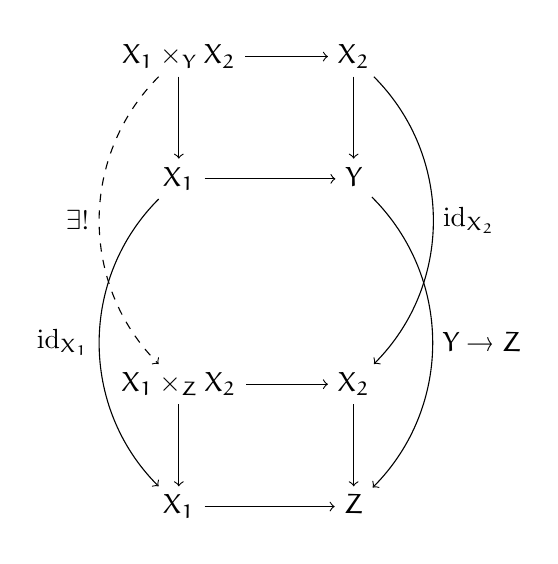
\begin{tikzpicture}[description/.style = {fill = white, inner sep = 2pt}, baseline=(current bounding  box.center)]
      \matrix (m) [matrix of math nodes, row sep = 3em, column sep = 3em, text height = 1.5ex, text depth = 0.25ex]
      {
        X_1\times_Y X_2 & X_2 \\
        X_1 & Y \\
        & \\
        X_1\times_Z X_2 & X_2 \\
        X_1 & Z \\
      };
      \path[->] (m-1-1) edge (m-1-2) (m-1-2) edge (m-2-2)
                (m-1-1) edge (m-2-1) (m-2-1) edge (m-2-2)
                (m-4-1) edge (m-4-2) (m-4-2) edge (m-5-2)
                (m-4-1) edge (m-5-1) (m-5-1) edge (m-5-2);
      \path[->] (m-1-2) edge[bend left = 45]  node[auto] {$\identity_{X_2}$} (m-4-2)
                (m-2-1) edge[bend right = 45] node[left] {$\identity_{X_1}$} (m-5-1)
                (m-2-2) edge[bend left = 45]  node[auto] {$Y\to Z$}          (m-5-2);
      \path[->, dashed] (m-1-1) edge[bend right = 45] node[left] {$\exists!$} (m-4-1);
                
    \end{tikzpicture}
  \end{equation}
  as all maps agree by taking the compositions and we can use the definition of the fibered diagram to obtain the unique map~$X_1\times_Y X_2\to X_1\times_Z X_2$.
\end{exercise}

\begin{exercise}
  Let's draw another picture.
  \begin{equation}
    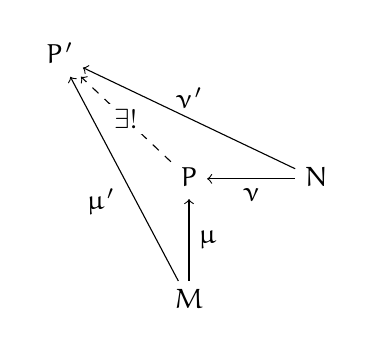
\begin{tikzpicture}[description/.style = {fill = white, inner sep = 2pt}, baseline=(current bounding  box.center)]
      \matrix (m) [matrix of math nodes, row sep = 3em, column sep = 3em, text height = 1.5ex, text depth = 0.25ex]
      {
        P' & & \\
        & P & N \\
        & M & \\
      };
      \path[->] (m-2-3) edge node[above] {$\nu'$} (m-1-1)
                (m-3-2) edge node[auto] {$\mu'$} (m-1-1)
                (m-2-3) edge node[auto] {$\nu$} (m-2-2)
                (m-3-2) edge node[right] {$\mu$} (m-2-2);
      \path[->, dashed] (m-2-2) edge node[description] {$\exists!$} (m-1-1);
    \end{tikzpicture}
  \end{equation}

  When~$P=M\sqcup N$ we have obvious morphisms~$\mu$ and~$\nu$ which are the canonical injections. But~$\mu'$ and~$\nu'$ are uniquely determining~$P\to P'$ as exactly the right information is stored in~$P$.
\end{exercise}

\begin{exercise}
  We check the axioms for the ring morphism~$b\mapsto b\otimes 1$:
  \begin{description}
    \item[additivity] By definition of the tensor product of two~$A$\nobreakdash-modules we obtain
      \begin{equation}
        (b_1+b_2)\otimes c=b_1\otimes c+b_2\otimes c,
      \end{equation}
      hence the map is additive.  
    \item[multiplicativity] By the definition of multiplication induced on~$B\otimes_A C$ in~\autoref{exercise:23k} we obtain~$(b_1b_2)\otimes 1=(b_1\otimes 1)(b_2\otimes 1)$.

    \item[preservation of unity] By definition we have~$1\mapsto 1\otimes 1$ which acts as unity for the multiplication.
  \end{description}

  We have maps~$B\to B\otimes_A C$ and~$C\to B\otimes_A C$ by the previous observations. Now these maps agree by definition of~$\otimes_A$: the images of elements of~$A$ in either~$B$ or~$C$ can be moved back and forth after the map to~$B\otimes_A C$.

  For any other ring~$A'$ equipped with maps~$f\colon B\to A'$ and~$g\colon C\to A'$ such that they agree when composed with~$A\to B$ and~$A\to C$ we have an obvious map~$B\otimes_A C\to A'$ by taking~$b\otimes c\mapsto f(b)g(c)$. As unity is preserved under ring morphisms, this makes everything commute. By the axioms of ring morphisms, this is the unique map making everything commute as this multiplicative structure of the map is imposed.
\end{exercise}

\begin{exercise}
  Consider two maps~$g_1,g_2\colon Z\to X$ and two consecutive mono\-morphisms~$f_1\colon X\to Y_1$,~$f_2\colon Y_1\to Y_2$ such that~$f_2\circ f_1\circ g_1=f_2\circ f_1\circ g_2$, by associativity and~$f_2$ monomorphic we obtain~$f_1\circ g_1=f_1\circ g_2$ which by~$f_1$ monomorphic yields~$g_1=g_2$.
\end{exercise}

\begin{exercise}
  \label{exercise:23v}
  If~$f\colon X\to Y$ is a monomorphism taking~$X$ as the fibered product proves its existence. The unique map~$Z\to X\times_Y X=X$ is given by~$g_1=g_2$, where~$g_1,g_2\colon Z\to X$.

  Conversely, if the fibered product exists we have that~$f\circ g_1=f\circ g_2$ as these maps must agree. Now there is a \emph{unique} map~$Z\to X\times_Y X$ so we obtain~$g_1=g_2$ as~$g_1$ and~$g_2$ both equal the composition of this unique map with the equal projections~$X\times_Y X\to X$.

  By putting~$X$ in the position for a map~$X\to X\times_Y X$ we obtain an induced isomorphism as we can use the identity map~$X\to X$ at both sides in the diagram.
\end{exercise}

\begin{exercise}
  Using the magic diagram we obtain
  \begin{equation}
    \begin{tikzpicture}[description/.style = {fill = white, inner sep = 2pt}, baseline=(current bounding  box.center)]
      \matrix (m) [matrix of math nodes, row sep = 3em, column sep = 3em, text height = 1.5ex, text depth = 0.25ex]
      {
        X_1\times_Z X_2 & & \\
        & X_1\times_Y X_2 & X_1\times_Z X_2 \\
        & Y & Y\times_Z Y\cong Y \\
      };
      \path[->] (m-1-1) edge (m-3-2)
                (m-1-1) edge (m-2-3)
                (m-2-2) edge (m-3-2)
                (m-2-2) edge (m-2-3)
                (m-3-2) edge (m-3-3)
                (m-2-3) edge (m-3-3);
      \path[->, dashed] (m-1-1) edge (m-2-2);
    \end{tikzpicture}
  \end{equation}
  where we have~$Y\times_Z Y\cong Y$ by~\autoref{exercise:23v}. The isomorphism is immediate by the uniqueness of~$X_1\times_Z X_2\to X_1\times_Y X_2$.
\end{exercise}

\begin{exercise}
  By plugging in~$C=A$ we get the candidate~$g\colonequals\mathrm{i}_A(\identity_A)$. 
\end{exercise}


\section{Limits and colimits}

\begin{exercise}
  As stated in the exercise the morphisms~$f_j$ are the obvious projection maps. The maps~$F(m)$ for all~$m\colon j\to k$ in~$\mathcal{I}$ commute with these projections by the identification~$F(m)(a_j)=a_k$.

  Now take an object~$W$ such that the~$g_i\colon W\to A_i$ commute with all the~$F(m)$. Construct~$g\colon W\to\varprojlim_{\mathcal{I}}A_i$ by using he value~$g_i(w)$ for the~$i$th position of the direct limit. By demanding commutativity this map is necessarily unique.
\end{exercise}

\begin{exercise}
  \label{exercise:24b}
  \begin{enumerate}
    \item The rational numbers~$\mathbb{Q}$ is the object that captures all of the information contained in the~$\frac{1}{n}\mathbb{Z}$. We define a morphism~$\frac{1}{n}\mathbb{Z}\to\frac{1}{m}\mathbb{Z}$ is~$n\divides m$, by~$\frac{z}{n}\mapsto\frac{(m/n)z}{m}$. The remark in the notes after~\autoref{exercise:24c} is helpful in this respect.

    \item\label{enumerate:24-b} Take subsets~$A_j$ and~$A_k$ of~$A$ such that~$m\colon A_j\hookrightarrow A_k$ is the obvious inclusion map (if it exists). The diagram becomes
      \begin{equation}
        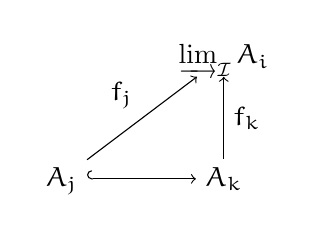
\begin{tikzpicture}[description/.style = {fill = white, inner sep = 2pt}, baseline=(current bounding  box.center)]
          \matrix (m) [matrix of math nodes, row sep = 3em, column sep = 3em, text height = 1.5ex, text depth = 0.25ex]
          {
            & \varinjlim_{\mathcal{I}}A_i \\
            A_j & A_k \\
          };
          \path[->] (m-2-1) edge node[auto] {$f_j$} (m-1-2)
                    (m-2-2) edge node[right] {$f_k$} (m-1-2);
          \path[right hook->] (m-2-1) edge (m-2-2);
        \end{tikzpicture}
      \end{equation}
      where~$\varinjlim_{\mathcal{I}}A_i$ should capture enough but no more of the information contained in the~$A_i$ in order to make maps out of it to compatible objects unique.

      Therefore two different elements are mapped to different elements of the colimit, but they are identified for the inclusion maps. The union captures all of this information: we have the obvious inclusions~$f_i$, the~$F(m)$ are still the inclusion maps from the previous paragraph and as to maps out of~$\varinjlim_{\mathcal{I}}A_i$ to compatible objects: these are unique because the~$g_j$ define them uniquely.
  \end{enumerate}
\end{exercise}

\begin{exercise}
  \label{exercise:24c}
  Extending the answer to~\autoref{exercise:24b}\ref{enumerate:24-b} we see that the maps out of~$\varinjlim_{\mathcal{I}}A_i$ are defined uniquely by this quotient of the disjoint union.
\end{exercise}

\begin{exercise}
  First the well-definedness:
  \begin{description}
    \item[addition] the pointwise addition is compatible with the construction because the maps are all~$A$\nobreakdash-module maps, hence the identification is preserved;
    \item[scalar multiplication] the same reasoning holds.
  \end{description}

  And this construction serves as a colimit because two elements that get identified will have an equal image out of the colimit (\ie, just one choice) while the compatibility of the maps gives us the construction of the map~$\varinjlim_{\mathcal{I}}\to W$\footnote{You might have noticed it: I am not god at this kind of arguments. Please consult a good algebra textbook.}.
\end{exercise}

\begin{exercise}
  The maps~$F(m)\colon\frac{1}{s_1}A\to\frac{1}{s_2}A$ where~$s_2=s_1s'$ are defined by~$\frac{1}{s_1}a\mapsto\frac{1}{s_2}s'a$. So an element in~$S^{-1}A$ which can be regarded as a fraction appears somewhere in the direct system and stays there by the integrality. The direct limit essentially captures all the information of the localization, for which integral domains are the most intuitive case.

  In this more general case, the torsion will disappear.
\end{exercise}

\begin{exercise}
  The diagram defining the colimit is now broken into several disjoint parts by lack of the filtered condition. The construction works for these parts and they are independent, hence these are not affected by the quotient of the direct sum.
\end{exercise}


\section{Adjoints}

\begin{exercise}
  \label{exercise:25a}
  Extending the diagram given in~(2.5.0.2) we obtain
  \begin{equation}
    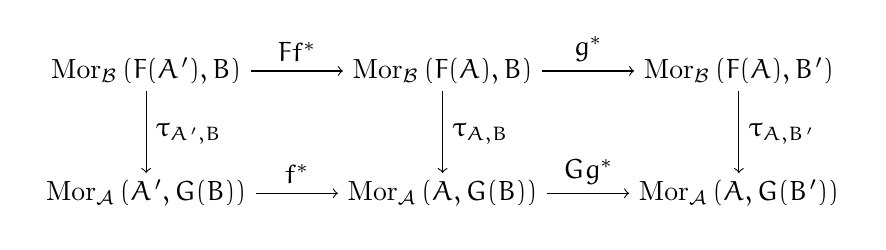
\begin{tikzpicture}[description/.style = {fill = white, inner sep = 2pt}, baseline=(current bounding  box.center)]
      \matrix (m) [matrix of math nodes, row sep = 3em, column sep = 3em, text height = 1.5ex, text depth = 0.25ex]
      {
        \Mor_{\mathcal{B}}\left( F(A'),B \right) & \Mor_{\mathcal{B}}\left( F(A),B \right) & \Mor_{\mathcal{B}}\left( F(A),B' \right) \\
        \Mor_{\mathcal{A}}\left( A',G(B) \right) & \Mor_{\mathcal{A}}\left( A,G(B) \right) & \Mor_{\mathcal{A}}\left( A,G(B') \right) \\
      };
      \path[->] (m-1-1) edge node[auto] {$Ff^*$} (m-1-2)
                (m-1-2) edge node[auto] {$g^*$}  (m-1-3)
                (m-2-1) edge node[auto] {$f^*$}  (m-2-2)
                (m-2-2) edge node[auto] {$Gg^*$} (m-2-3)
                (m-1-1) edge node[auto] {$\tau_{A',B}$} (m-2-1)
                (m-1-2) edge node[auto] {$\tau_{A,B}$}  (m-2-2)
                (m-1-3) edge node[auto] {$\tau_{A,B'}$} (m-2-3);
    \end{tikzpicture}
  \end{equation}
  in an obvious way, where~$g^*$ is \emph{appending} the morphism to~$f\colon F(A)\to B$.
\end{exercise}

\begin{exercise}
  The map~$\eta_A$ should behave somewhat like an identity. If we take
  \begin{equation}
    \eta_A\colonequals\tau_{A,F(A)}^{-1}\left( \identity_{F(A)} \right) 
  \end{equation}
  with~$\identity_{F(A)}\in\Mor_{\mathcal{B}}(F(A),F(A))$ we find the correct definition.
  
  Analogously we take
  \begin{equation}
    \epsilon_B\colonequals\tau_{G(B),B}^{-1}\left( \identity_{G(B)} \right)
  \end{equation}
  in~$\Mor_{\mathcal{A}}(G\circ F(A),A)$ where~$\identity_{G(B)}\in\Mor_{\mathcal{A}}(G(B),G(B))$.

  Now these maps are the ones we were looking by the functoriality of~$F$ and~$G$.
\end{exercise}

\begin{exercise}
  Taking~$f\colon M\otimes_A N\to P$, transform it to~$g\colon M\to\Hom_A(N,P)$ by defining~$g(m)(-)\colonequals f(m\otimes-)$. This is a bijection:
  \begin{description}
    \item[injective] Take~$f_1,f_2$ such that~$f_1\neq f_2$, \ie, there exist~$m\in M$ and~$n\in N$ such that~$f_1(m\otimes n)\neq f_2(m\otimes n)$. Taking the corresponding~$g_i$ we obtain~$g_1(m)(-)\neq g_2(m)(-)$ as their values in the point~$n$ differ.

    \item[surjective] By the universal property of the tensor product.
  \end{description}
\end{exercise}

\begin{exercise}
  \label{exercise:25d}
  It just boils down to unwinding the diagram from~\autoref{exercise:25a}. Set~$F\colonequals-\otimes_A N$ and~$G\colonequals\Hom_A(N,-)$, $A\colonequals M$, $A'\colonequals M'$, $B\colonequals P$ and~$B'\colonequals P'$. Now taking~$h\colon M'\otimes_A N\to P$, chasing the diagram using~$\tau_{A,B}\circ Ff^*$ we obtain~$h\circ (f\otimes\identity)(-_M\otimes-_N)$ first and then~$h(f(-_M))(-_N)$.

  Chasing the diagram in the other direction, through~$f^*\circ\tau_{A',B}$ we first obtain~$h(-_M)(-_N)$ and then end up with~$h(f(-_M))(-_N)$, hence equality. The rest is analogous, now you have to compose with the map~$g\colon B\to B'$.
\end{exercise}

\begin{exercise}
  Let's take the equivalence relation described in the notes with \emph{pointwise addition}. Now we check the group axioms:
  \begin{description}
    \item[closure] taking~$(a,b)$ and~$(c,d)$ in~$S\times S$, the pointwise sum is~$(a+c,d+e)$ and both components are defined by the binary operation in the semigroup;
    \item[associativity] again, the pointwise sum is associative by the associativity of the binary operation in the semigroup;
    \item[identity] the element~$(s,s)$ for~$s\in S$ is the identity: all of them are identified by the equivalence relation and we have~$(a,b)\sim(a+s,b+s)$ because~$a+b+s+e=b+a+s+e$ as~$S$ is an \emph{abelian} semigroup;
    \item[inverse element] the inverse element of~$(a,b)$ is given by~$(b,a)$: their sum is~$(a+b,b+a)$ which is a representative of the equivalence class of the identity.
  \end{description}

  The map~$S\to\groupification(S)$ is given by choosing a fixed element~$e$ and mapping~$s$ to~$\overline{(s,e)}$ in~$S\times S/{\sim}$. By the equivalence relation, any choice will do and induce the same abelian group.

  Reproducing the diagram for~\autoref{exercise:25a} with the corresponding functors in place we obtain
  \begin{equation}
    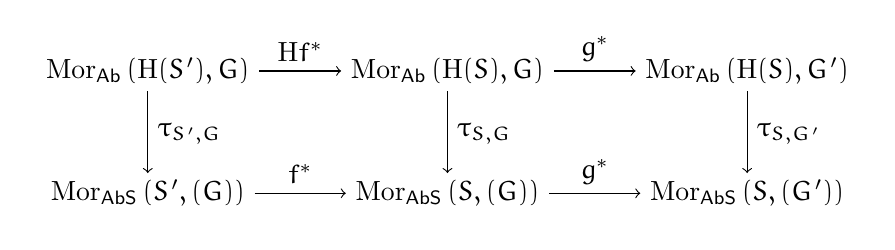
\begin{tikzpicture}[description/.style = {fill = white, inner sep = 2pt}, baseline=(current bounding  box.center)]
      \matrix (m) [matrix of math nodes, row sep = 3em, column sep = 3em, text height = 1.5ex, text depth = 0.25ex]
      {
        \Mor_{\category{Ab}}\left( \groupification(S'),G \right) & \Mor_{\category{Ab}}\left( \groupification(S),G \right) & \Mor_{\category{Ab}}\left( \groupification(S),G' \right) \\
        \Mor_{\category{Ab S}}\left( S',\forgetful(G) \right) & \Mor_{\category{Ab S}}\left( S,\forgetful(G) \right) & \Mor_{\category{Ab S}}\left( S,\forgetful(G') \right) \\
      };
      \path[->] (m-1-1) edge node[auto] {$\groupification f^*$} (m-1-2)
                (m-1-2) edge node[auto] {$g^*$}  (m-1-3)
                (m-2-1) edge node[auto] {$f^*$}  (m-2-2)
                (m-2-2) edge node[auto] {$\forgetful g^*$} (m-2-3)
                (m-1-1) edge node[auto] {$\tau_{S',G}$} (m-2-1)
                (m-1-2) edge node[auto] {$\tau_{S,G}$}  (m-2-2)
                (m-1-3) edge node[auto] {$\tau_{S,G'}$} (m-2-3);
    \end{tikzpicture}
  \end{equation}
  where~$f\colon S\to S'$ in~$\category{Ab S}$ and~$g\colon G\to G'$ in~$\category{Ab}$. The maps~$\tau_{S,G}$ are obtained by forgetting the group structure on~$\groupification(S)$, \ie, given~$m\colon\groupification(S)\to G$ we let~$\tau_{S,G}m$ be the map sending~$s\in S$ to the image of~$\overline{(s,e)}$ under~$m$ which is~$\overline{(m(s),m(e))}$.

  Now the commutativity follows from the following observation: taking a morphism~$n\colon\groupification(S')\to G$, applying~$\groupification f^*$ yields a map
  \begin{equation}
    \groupification f^*(g)\colon\overline{(s,e)}\mapsto g\left( \overline{\left( f(s),f(e) \right)} \right). 
  \end{equation}
  We immediately see that going the other direction is equal by definition of~$f^*$. The second part is completely analogous.
\end{exercise}

\begin{exercise}
  By filling in~$\pi=\identity_S$ in the universal property defining groupification we easily see the unique morphism~$G\to G'$ is given by~$S\to G$.
\end{exercise}

\begin{exercise} % TODO prove adjointness
  Because by definition~$1\in S$ we have the desired inclusion of categories~$\category{Mod}_{S^{-1}A}\hookrightarrow\category{Mod}_A$ as every~$S^{-1}$\nobreakdash-module is an~$A$\nobreakdash-module using~$a\mapsto a/1$. The converse doesn't hold obviously.

  Now this embedding is fully faithful: every~$A$\nobreakdash-module morphism~$M\to M'$ is an~$S^{-1}A$\nobreakdash-module morphism: the localization can occur either before or after the morphism by the corresponding linearity.

  The adjointness is still to come.
\end{exercise}


\section{(Co-)kernels and exact sequences (an introduction to abelian categories)}

\begin{exercise}
  By the Freyd-Mitchell embedding theorem, we can diagram-chase elements. By the element-wise definition of~$\image f^i$ there is an injection~$\image f^i\hookrightarrow A^{i+1}$ and likewise the cokernel is \emph{defined as}~$A^{i+1}/\image f^i$, hence we immediately obtain the surjection in the second part of the diagram.

  The~$i$th cohomology~$\homology^i(A^\bullet)$ is defined as~$\ker f^i/\image f^{i-1}$ which gives us the injection into~$\coker f^{i-1}$, defined as~$A^i/\image f^{i-1}$, by the injection~$\ker f^{i}\hookrightarrow A^i$. For the surjectivity of~$\coker f^{i-1}\to\image f^i$ we use the fact that it is a complex:~$f^i\circ f^{i-1}=0$.
\end{exercise}

\begin{exercise}
  We first use the fact from linear algebra that for the exact sequence
  \begin{equation}
    0\to A^1\to A^2\to A^3\to 0
  \end{equation}
  where~$\dim A^2=\dim A^1+\dim A^3$.

  Now by taking the long sequence apart and setting~$A^1\colonequals\image d^i=\ker d^{i+1}$ and likewise~$A^3\colonequals\image d^i=\ker d^{i+1}$ we can chain all these sums together and obtain the desired equality.
\end{exercise}

\begin{exercise}
  The key insight is: \emph{positionwise}. The category~$\category{Com}_{\category{Mod}_A}$ is additive by imposing the positionwise (as in: each position in a complex) structures. The kernels and cokernels of maps of complexes are defined by putting the appropriate (co)kernels at each position. The additional axioms of an abelian category follow likewise.
\end{exercise}

\begin{exercise} % TODO expand
  The truth lies in the commutativity of diagram~(2.6.4.5), but I have to come up with a good formulation.
\end{exercise}

\begin{exercise}
  This is by breaking apart the short exact sequences and putting them back together equivalent to the definition.
\end{exercise}

\begin{exercise}
  \begin{enumerate}
    \item We consider an exact sequence
      \begin{equation}
        0\to M'\to M\to M''\to 0 
      \end{equation}
      in~$\category{Mod}_A$ that is mapped by~$S^{-1}$ to a sequence
      \begin{equation}
        0\to S^{-1}M'\to S^{-1}M\to S^{-1}M''\to 0
      \end{equation}
      in~$\category{Mod}_{S^{-1}A}$ and we'll study its exactness.

      This is almost by definition: if we take a morphism~$f\colon M\to M'$ in~$\category{Mod}_A$ we define~$S^{-1}f\colon S^{-1}M\to S^{-1}M'$ to be~$S^{-1}f\colon (m/s)\mapsto (f(m)/s)$. The surjectivity is obviously preserved and if~$(m'_1/s),(m'_2/s)\in S^{-1}M'$ are two different element such that~$S^{-1}f(m'_1/s)=S^{-1}f(m'_2/s)$ we have that~$ss'(f(m'_1)-f(m'_2))=0$ but this implies~$f(m'_1)=f(m'_2)$, a contradiction.

    \item See~\autoref{exercise:23h}.

    \item Now considering the exact sequence
      \begin{equation}
        0\to M_1\to M_2\to M_3
      \end{equation}
      with~$f\colon M_1\to M_2$ and~$g\colon M_2\to M_3$ in~$\category{Mod}_A$, which is transformed to
      \begin{equation}
        0\to\Hom(M,M_1)\to\Hom(M,M_2)\to\Hom(M,M_3),
      \end{equation}
      in~$\category{Mod}_A$. The preservation of injectivity is satisfied by definition of a monomorphism: take~$g_1,g_2\colon m\to M_1$ such that the induced~$\Hom(M,f)$ maps these to~$f\circ g_1=f\circ g_2$, we have~$g_1=g_2$.

      Now for the exactness at~$\Hom(M,g)$, I was heavily inspired by~\href{http://math.stackexchange.com/questions/47401/hom-is-a-left-exact-functor}{this question at \texttt{math.stackexchange.com}} as my original proof looked quite like the asker's proof. We have~$\image f=\ker g$, so~$g\circ f=0$ and~$f$ has the universal property
      \begin{equation}
        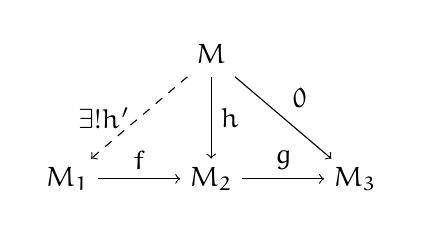
\begin{tikzpicture}[description/.style = {fill = white, inner sep = 2pt}, baseline=(current bounding  box.center)]
          \matrix (m) [matrix of math nodes, row sep = 3em, column sep = 3em, text height = 1.5ex, text depth = 0.25ex]
          {
            & M & \\
            M_1 & M_2 & M_3 \\
          };
          \path[->] (m-2-1) edge node[auto] {$f$} (m-2-2)
                    (m-2-2) edge node[auto] {$g$} (m-2-3)
                    (m-1-2) edge node[auto] {$h$} (m-2-2)
                    (m-1-2) edge node[auto] {$0$} (m-2-3);
          \path[->, dashed] (m-1-2) edge node[left] {$\exists!h'$} (m-2-1);
        \end{tikzpicture}
      \end{equation}
      where~$h\colon M\to M_2$ such that~$g\circ h=0$ and we obtain a factorization~$f\circ h'=h$. So if~$\Hom(M,g)(h)=0$ we have~$\Hom(M,f)(h')=0$ hence we obtain the first inclusion~$\ker\Hom(M,g)\subseteq\image\Hom(M,f)$ and~$\Hom(M,i)$ is injective.

      Now we draw the second diagram
      \begin{equation}
        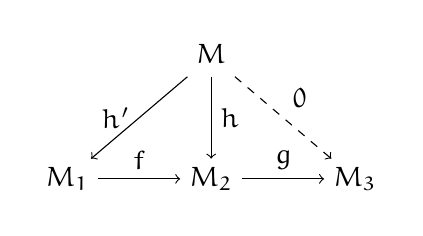
\begin{tikzpicture}[description/.style = {fill = white, inner sep = 2pt}, baseline=(current bounding  box.center)]
          \matrix (m) [matrix of math nodes, row sep = 3em, column sep = 3em, text height = 1.5ex, text depth = 0.25ex]
          {
            & M & \\
            M_1 & M_2 & M_3 \\
          };
          \path[->] (m-2-1) edge node[auto] {$f$}  (m-2-2)
                    (m-2-2) edge node[auto] {$g$}  (m-2-3)
                    (m-1-2) edge node[left] {$h'$} (m-2-1)
                    (m-1-2) edge node[auto] {$h$}  (m-2-2);
          \path[->, dashed] (m-1-2) edge node[auto] {$0$} (m-2-3);
        \end{tikzpicture}
      \end{equation}
      where~$h\colon M\to M_1$ is such that~$h=f\circ h'=\Hom(M,f)h'$ we easily obtain~$\Hom(M,g)h=0$ because
      \begin{equation}
        \Hom(M,g)h=\Hom(M,g)\Hom(M,f)h'=\Hom(M,g\circ f)h'=0\circ f
      \end{equation}
      so~$\image\Hom(M,f)\subseteq\ker\Hom(M,g)$. We have obtained equality.

      The covariance is by the position of~$M$: a morphism~$M\to M_1$ gives rise to a morphism~$M\to M_2$ by composing it on the right with~$M_1\to M_2$ (where composition on the right means ``on the right in the diagram'', it's on the left when notated as functions).

      And finally: the proof holds in general abelian categories, we have not assumed anything about a module structure on our objects.

    \item The proof of the left-exactness of~$\Hom(M,\cdot)$ can be adapted to proof right-exactness of~$\Hom(\cdot,M)$, noting that we have contravariance: given~$M_2\to M$ we obtain a morphism~$M_1\to M$ by composing it on the left.
  \end{enumerate}
\end{exercise}


\chapter{Sheaves}
\section{Motivating example: the sheaf of differentiable functions}

\begin{exercise}
  As every element of~$\mathcal{O}_p\setminus\mathfrak{m}$ is nonzero in a neighbourhood of~$p$ we can restrict an element such that it is invertible there, a property which is preserved when taking the stalk. Hence the germ of a non-vanishing function is invertible and~$\mathfrak{m}$ is invertible.
\end{exercise}

\begin{exercise} % TODO find out what is asked for
  I don't really have a differential geometry background and I fail to see what should be proved. But I should revisit this exercise later.
\end{exercise}


\section{Definition of sheaf and presheaf}

\begin{exercise}
  A functor assigns an object in~$\category{Sets}$ to every object in the category of open sets of the topological space~$X$. As an inclusion of sets is reflected as a morphism of the two open sets involved, this is translated to a morphism of sets in the codomain category\footnote{I have never seen this terminology, don't shoot me if I missed some more obvious wording.}. Identities are preserved by functors, so~$\res_{U,U}=\identity_{\mathcal{F}(U)}$ by definition. For the commutativity of restriction maps, this is by the \emph{contravariance} of the functor.
\end{exercise}

\begin{exercise}
  \begin{enumerate}
    \item The presheaf axioms are (trivially) true by restriction of functions. Yet it is not a sheaf, take~$x\mapsto|x|$. On~$\ball(0,n)$ the function is bounded by~$n$, we can take~$\mathbb{C}=\bigcup_{n\in\mathbb{N}}\ball(0,n)$ and glue together a function on all of~$\mathbb{C}$ yet it is not bounded hence not a section over~$\mathcal{C}$ of this sheaf.

    \item Inspired by \href{http://math.stackexchange.com/questions/38423/presheaf-which-is-not-a-sheaf-holomorphic-functions-which-admit-a-holomorphic}{\texttt{math.stackexcange.com}} (and my complex analysis course) the idea is to circle a zero, ending up with a multiple-valued function, which is clearly not a section of the sheaf.

      Take~$f\colon z\mapsto z$ on the annulus~$U=\left\{ 1-\epsilon<|z|<1+\epsilon \right\}$. By the Cauchy integral formula we have
      \begin{equation}
        \oint_{\mathclap{|z|=1}}\frac{g'(z)}{g(z)}\dd z\in2\pi\mathrm{i}\mathbb{Z}
      \end{equation}
      where~$g$ is holomorphic, without zeroes on the unit circle. Hence for~$f$ we obtain~$2\pi\mathrm{i}$.

      But if~$f=g^2$ we would obtain
      \begin{equation}
        \oint_{\mathclap{|z|=1}}\frac{f'(z)}{f(z)}\dd z=2\oint_{\mathclap{|z|=1}}\frac{g'(z)}{g(z)}\dd z\in4\pi\mathrm{i}\mathbb{Z}
      \end{equation}
      which is a contradiction on the value we previously obtained. Now~$f$ can be patched together from holomorphic functions that admit a square root, as long as the open set doesn't wind around zero: take open balls to cover~$U$ and we're done.
  \end{enumerate}
\end{exercise}

\begin{exercise}
  As we have maps~$\mathcal{F}(\bigcup U_i)\to\mathcal{F}(U_i)$ (or arbitrary unions of~$U_i$) this is a limit: the arrows from our desired object map \emph{to} all the objects as described in~2.4.4.
\end{exercise}

\begin{exercise}
  \label{exercise:32d}
  \begin{enumerate}
    \item Such functions are defined in their points, if all the restrictions agree for a covering, the functions are obviously equal. The identity axiom is satisfied. But given a covering on which all restrictions agree we can just paste together a global function, hence the gluability axiom is satisfied~too.

      Glueing functions preserves their extra properties: these are all defined in a neighbourhood of a point, hence valid in an open set and therefore lift to the global function.

    \item Analogous.
  \end{enumerate}
\end{exercise}

\begin{exercise}
  The presheaf axioms are trivially satisfied, local functions restrict easily. The identity axiom is obvious too. For the gluability: observe that the compatibility boils down to defining a function on the \emph{connected components} of the covering because sections are constant if there is a non-empty intersection and therefore this axiom is satisfied too.
\end{exercise}

\begin{exercise}
  \label{exercise:32f}
 The key idea is ``a function is continuous'' if and only if ``locally a function is continuous''. Hence restriction of continuous functions is well defined and the commutativity of the restriction triangle is immediate. Now for the identity axiom: equality of functions is checked in the points and as all restrictions agree the global sections must agree. Likewise we can check the gluability axiom.
\end{exercise}

\begin{exercise}
  \begin{enumerate}
    \item The sections of~$f$ over~$U$ form a subset of the sections of the sheaf from~\autoref{exercise:32f} over~$U$. The restrictions are trivially fine, the identity axiom follows from the previous exercise too and gluability is obviously true as well as~$f\circ s=\identity|_U$ holds for the pointwise glueing of a section.

    \item There is nothing to add to the arguments of~\autoref{exercise:32d}. The set of sections carries a natural pointwise abelian group structure.
  \end{enumerate}
\end{exercise}

\begin{exercise}
  The presheaf axioms are satisfied because~$f$ is continuous hence the inverse~$f^{-1}$ maps open sets to open sets. The presheaf axioms are satisfied on the open sets in the domain of the map and the presheaf axioms for~$f_*\mathcal{F}$ are a subset (sketchy wording) of those for~$\mathcal{F}$.

  The sheaf axioms are satisfied because inverse maps are compatible with unions and intersections. As for the presheaf axioms: everything is transferred.
\end{exercise}

\begin{exercise}
  Using the definition of the direct limit and the construction as described in~\autoref{exercise:23c} we see that \emph{less} relations have to be quotiented, as the direct system defining~$(f_*\mathcal{F})_y$ is contained in the direct system defining~$\mathcal{F}_p$.
\end{exercise}

\begin{exercise}
  As germs in the stalk~$\mathcal{F}_x$ are equivalence classes of functions defined in the neighbourhood modulo equality on a (smaller) neighbourhood, we can define the~$\mathcal{O}_{X,x}$\nobreakdash-module structure on~$\mathcal{F}_x$ by defining it on representatives of these classes. By commutativity of~(3.2.12.1) this is well defined. The actual checking of the structure is straightforward and familiar.
\end{exercise}


\section{Morphisms of presheaves and sheaves}

\begin{exercise}
  The induced morphism is given by applying the morphism to representatives of equivalence classes of the stalks. By commutativity of the diagram in the definition of (pre)sheaf morphisms this is correct.
\end{exercise}

\begin{exercise}
  To every sheaf~$\mathcal{F}$ in~$\category{Sets}_X$ there is a (unique) associated sheaf~$f_*(\mathcal{F})$ in~$\category{Sets}_Y$. Obviously~$f_*(\identity_\mathcal{F})=\identity_{f_*(\mathcal{F})}$ and we have~$f_*(h\circ g)$ with~$g\colon\mathcal{F}\to\mathcal{G}$ and~$h\colon\mathcal{G}\to\mathcal{H}$ by applying this to every open set~$U$.
\end{exercise}

\begin{exercise}
  The presheaf axioms are easy: the associated restriction is just the obvious restriction of a function~$f\colon\mathcal{F}(U)\to\mathcal{G}(U)$ to~$f|_V\colon\mathcal{F}(V)\to\mathcal{G}(V)$ in~$\SheafHom(\mathcal{F},\mathcal{G})(V)$ for~$V\subseteq U$.

  The identity axiom for~$\SheafHom$ follows from the separatedness of~$\mathcal{G}$. Take a cover~$(U_i)_i$ of~$U$, any open subset~$V$ of~$U$ and a section~$s\in\mathcal{F}(V)$. Now we have~$f(V)(s)|_{U_i\cap V}=g(V)(s)|_{U_i\cap V}$ (which are elements of the sheaf~$\mathcal{G}$) for the covering~$(U_i\cap V)_i$ of~$V$. As~$\mathcal{G}$ is assumed to be separated we obtain~$f(V)(s)=g(V)(s)$. As this holds for any~$V$ and all sections~$s$, we have that~$\SheafHom$ is a separated presheaf.

  Now consider a family~$(f_i)_i$ of compatible sections (which are morphisms of sets of sections) on a cover~$(U_i)_i$ of~$U$. Like the case of the identity axiom, we consider~$V\subseteq U$ open and~$s\in\mathcal{F}(V)$. This gives
  \begin{equation}
    f_i(U_i\cap V)(s|_{U_i\cap V})\in\mathcal{G}(U_i\cap V).
  \end{equation}
  Now glue together~$f(V)(s)$ in~$\mathcal{G}(V)$. This defines a morphism of presheaves, by separatedness of~$\mathcal{G}$ (the compatibility of restrictions is induced in a unique way).

  If~$\mathcal{G}$ is a sheaf of abelian groups, morphisms~$\mathcal{F}\to\mathcal{G}$ carry a natural group structure, by pointwise addition. The neutral element is the zero map.
\end{exercise}

\begin{exercise}
  \begin{enumerate}
    \item By definition
      \begin{equation}
        \SheafHom\left( \underline{\left\{ p \right\}},\mathcal{F} \right)=\Mor\left( \underline{\left\{ p \right\}}|_U=\left\{ p \right\},\mathcal{F}|_U \right).
      \end{equation}
      As there is a unique map~$f_x\colon\left\{ p \right\}\to\mathcal{F}|_U:p\mapsto x$ for every element of~$x\in\mathcal{F}|_U$ (hence a bijection of sets) we have obtained an isomorphism of sheaves.

    \item\label{enumerate:exercise-33d-b} Analogously we now have a map~$f_g\colon\underline{\mathbb{Z}}(U)=\mathbb{Z}\to\mathcal{F}(U)$ such that~$1\mapsto g$, defined for every~$g\in\mathcal{F}(U)$. Now take sections~$g$ and~$g'\in\mathcal{F}(U)$. We obtain~$f_{g+g'}=f_g+f_{g'}$ because the image of~$1$ defines everything (\ie,~$\mathbb{Z}$ is the free group generated by~$\left\{ 1 \right\}$).

    \item Analogous to~\ref{enumerate:exercise-33d-b}.
  \end{enumerate}
\end{exercise}

\begin{exercise}
  In the situation of the diagram as given in the notes, we have injective maps~$\ker_{\textrm{pre}}\phi(V)\to\mathcal{F}(V)$ for every~$V$ open. Define~$\res^{\ker}_{V,U}$ by mapping~$g\in\ker_{\textrm{pre}}\phi(V)$ to the preimage of~$\res_{V,U}$ under the injection maps. As both maps are injective, this preimage is a well-defined element. We have found our induced restriction map. It is unique by commutativity of the square and the injectivity: any two maps such that~$f\circ g_1=f\circ g_2$ imply~$g_1=g_2$.

  We now check the conditions required for a presheaf. Obviously~$\res^{\ker}_{U,U}$ is the identity map and the commutativity of the restriction triangle follows from the uniqueness of the restriction maps.
\end{exercise}

\begin{exercise}
  Given a presheaf morphism~$\phi\colon\mathcal{F}\to\mathcal{G}$, we would like to characterize~$\coker_{\textrm{pre}}f$ by the universal property
  \begin{equation}
    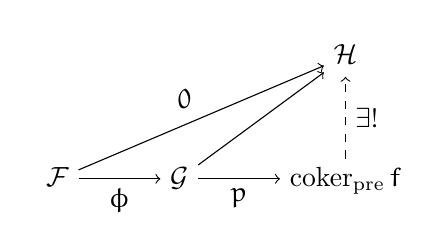
\begin{tikzpicture}[description/.style = {fill = white, inner sep = 2pt}, baseline=(current bounding  box.center)]
      \matrix (m) [matrix of math nodes, row sep = 3em, column sep = 3em, text height = 1.5ex, text depth = 0.25ex]
      {
        & & \mathcal{H} \\
        \mathcal{F} & \mathcal{G} & \coker_{\textrm{pre}}f \\
      };
      \path[->] (m-2-1) edge node[below] {$\phi$} (m-2-2)
                (m-2-2) edge node[below] {$p$}    (m-2-3)
                (m-2-1) edge node[auto]  {$0$}    (m-1-3)
                (m-2-2) edge                      (m-1-3);
      \path[->, dashed] (m-2-3) edge node[right] {$\exists!$} (m-1-3);
    \end{tikzpicture}.
  \end{equation}

  Defining~$(\coker_{\textrm{pre}}\phi)(U)\colonequals\coker\phi(U)$, we can conclude that the universal property characterizes this definition because categorical properties of presheaves and presheaf morphisms are verified on open sets. The map~$p$ is induced by the definition and the map~$\coker_{\textrm{pre}}\phi$ exists by the ``check on open sets'' mantra and is unique for the same reason.
\end{exercise}

\begin{exercise}
  \label{exercise:33g}
  A morphism between sheaves is defined as a morphism of the category over which we are considering the sheaf for \emph{every} open set. We now restrict ourselves to a specific open set, hence the morphisms (the only nontrivial part of a functor's definition) are preserved. 

  This functor is exact because the exactness of a sequence of sheaves if checked over open sets by the fact that all abelian-categorical notions are verified ``open set by open set''. And we only consider a specific open set, over which the exactness is given.
\end{exercise}

\begin{exercise}
  The abelian-categorial notions are verified ``open set by open set'', hence we consider a family of functors as in~\autoref{exercise:33g} indexed by all open sets in the topology on~$X$. The equivalence follows.
\end{exercise}

\begin{exercise} % TODO finish
  The uniqueness of the induced restriction map and the injectivity for every open set give us the identity axiom: if all restrictions are equal we can just move everything one morphism to the right and identify things there. The same holds for the gluability axiom: given local~$f_i$, we move everything using the injectivity to the sheaf's object~$\mathcal{F}(U_i)$ and lift things to~$\mathcal{F}(U)$. Now we don't now yet that this section lives in~$\ker_{\textrm{pre}}\phi$, but if it wouldn't, there needs to be an open set for which the image under~$\phi$ is nonzero. % TODO
\end{exercise}

\begin{exercise} % TODO finish
  The inclusion~$\underline{\mathbb{Z}}\hookrightarrow\mathcal{O}_X$ is obvious: constant functions are holomorphic. Under the mapping~$f\mapsto\exp(2\pi\mathrm{i}f$ the kernel are exactly those functions such that~$\exp(2\pi\mathrm{i}f)$ is~$1$ (the neutral element in this multiplicative group). This is true for all constant integer functions:~$2\pi\mathrm{i}n$ evaluates under exponentiation to~$1$. As~$\mathcal{F}$ is the presheaf of functions admitting a holomorphic logarithm, they must come from the exponentiation of a holomorphic function contained in~$\mathcal{O}_X$ and we have the surjectivity of~$\mathcal{O}_X\twoheadrightarrow\mathcal{F}$.

  The failure of the sheaf axioms is for tomorrow.
\end{exercise}


\section{Properties determined at the level of stalks, and sheafification}

\begin{exercise}
  Assume the map is not injective, \ie, there are sections~$f$ and~$g$ in~$\mathcal{F}(U)$ such that the product of their values in the stalks in~$U$ is equal. Every value arises by construction from a section on a neighbourhood, hence for the intersection of these neighbourhoods the restrictions of~$f$ and~$g$ have to agree. Now use the identity axiom because~$\mathcal{F}$ is a separated presheaf, which leads to~$f=g$, a contradiction.
\end{exercise}



\part{Schemes}

\chapter{Toward affine schemes}
\section{Toward schemes}

\begin{exercise} % TODO do this
  I should be ashamed of myself, not being able to answer this question.
\end{exercise}

\begin{exercise} % TODO do this
  I should be ashamed of myself, not being able to answer this question.
\end{exercise}


\section{The underlying set of affine schemes}

\begin{exercise}
  \label{exercise:42a}
  \begin{enumerate}
    \item\label{enumerate:42a-a} So we're looking for the prime ideals of~$\Spec k[\epsilon]/(\epsilon^2)$. But these correspond to the prime ideals of~$\Spec k[\epsilon]$ containing~$(\epsilon^2)$. Now the only prime ideal of this form is~$(\epsilon)$. This corresponds to the polynomials in~$\epsilon$ with no constant term. If there would be a constant term, \ie, something of the form~$a+b\epsilon$ it would be invertible modulo~$\epsilon^2$ using a geometric series. There is only one point.

      Notice that~$\Spec k[\epsilon]/(\epsilon)$ is not an integral domain:~$\epsilon^2$ is contained in~$(0)$ yet~$\epsilon\notin(0)$.

    \item\label{enumerate:42a-b} By commutative algebra the prime ideals of the localization correspond to the prime ideals of~$\Spec k[x]$ not containing~$(x)$. So the set~$\Spec k[x]_{(x)}$ corresponds to~$\Spec k[x]\setminus\left\{ (x) \right\}$ because there is only one prime ideal containing~$x$ namely~$(x)$: if there would be another one we could reduce it to a constant ending up the whole ring, a contradiction.
  \end{enumerate}
\end{exercise}

\begin{exercise}
  Using the discriminant we obtain the two roots of the quadratic which look like
  \begin{equation}
    x_{1,2}=\frac{-a\pm\sqrt{a^2-4b}}{2}
  \end{equation}
  where~$a^2-4b<0$. Now using operations of~$\mathbb{R}$ we can reduce this to~$i$.
\end{exercise}

\begin{exercise}
  This set corresponds to all polynomials that are irreducible over~$\mathbb{Q}$. There are the obvious points~$(x-a)$ where~$a\in\mathbb{Q}$, but all roots of polynomials are present too but they are glued together by the corresponding Galois actions. It corresponds to the identification of roots in the algebraic closure~$\mathbb{Q}^{\alg}$.
\end{exercise}

\begin{exercise}
  Suppose~$\mathfrak{p}$ is a prime ideal that is not a principal ideal. Take two essential generators~$f(x,y)$ and~$g(x,y)$ (\ie, with not all factors of one contained in the other). This must be possible because otherwise we wouldn't have a principal ideal: one can be written as a product of the other with a polynomial containing the missing factors. Now because~$\mathfrak{p}$ is prime we can remove all common factors.

  By applying the Euclidean algorithm in~$\mathcal{C}(x)[y]$ we can find a polynomial in the variable~$x$ contained in~$(f(x,y),g(x,y))\subseteq\mathfrak{p}$, which by the algebraic closedness of~$\mathcal{C}$ reduces to a linear factor~$(x-a)$ contained in~$\mathfrak{p}$ and analogously~$(y-b)\in\mathfrak{p}$.

  Obviously any principal ideal must be generated by an irreducible polynomial. So having reduced all non-principal ideals to ideals of the form~$(x-a,y-b)$ we have finished the proof.
\end{exercise}

\begin{exercise}
  The first maximal ideal is~$(x^2+y^2-4,x-y)$ while the second is~$(x^2+y^2-4,x+y)$. The residue fields are~$\mathbb{Q}(\sqrt{2})$ in both cases: substituting the second generator in the first yields this result.
\end{exercise}

\begin{exercise} % TODO do this
  I'm still wondering whether my answer is correct.
\end{exercise}

\begin{exercise}
  \label{exercise:42g}
  I have used this fact in~\autoref{exercise:42a}\ref{enumerate:42a-a}. It boils down to
  \begin{equation}
    A/J\cong (A/I)/(J/I) 
  \end{equation}
  where~$I\subseteq J$ are prime ideals of~$A$, and this is equivalent to~$\overline{J}$ being prime in~$A/I$.
\end{exercise}

\begin{exercise} % TODO rewrite this
  \label{exercise:42h}
  I have used this fact in~\autoref{exercise:42a}\ref{enumerate:42a-b}. A prime ideal of~$A$ that contains an element of~$S$ will the whole become~$S^{-1}A$ under localization. A prime ideal of~$A$ disjoint of~$S$ remains prime because the product~$(p_1/s_1)(p_2/s_2)$ is in the prime ideal if and only if~$(p_1p_2)/(s_1s_2)$ is in the prime ideal, but we can multiply with~$s_1s_2$ as this is by multiplicativity of~$S$ not a member of the prime ideal. Now we have reduced it to~$p_1p_2$ in the prime ideal.
\end{exercise}

\begin{exercise} % TODO do this
  I haven't figured it out yet.
\end{exercise}

\begin{exercise}
  Assume~$b_1b_2\in\phi^{-1}(\mathfrak{p})$, we have
  \begin{equation}
    \phi(b_1b_2)=\phi(b_1)\phi(b_2)\in\phi\left( \phi^{-1}(\mathfrak{p}) \right)=\mathfrak{p},
  \end{equation}
  hence~$\phi(b_1)$ or~$\phi(b_2)$ as~$\phi(\phi^{-1}(\mathfrak{p}))=\mathfrak{p}$ is a prime ideal in~$A$. We obtain that~$\phi^{-1}(\phi(b_1))=b_1$ or~$\phi^{-1}(\phi(b_2))=b_2$ must be an element of~$\phi^{-1}(\mathfrak{p})$.
\end{exercise}

\begin{exercise}
  \label{exercise:42k}
  \begin{enumerate}
    \item\label{enumerate:42k-a} Using~\autoref{exercise:42g} everything is already clear: the primes of~$A$ containing~$I$ form a subset of~$\Spec A$ and~$\phi^{-1}$ is an inclusion-preserving bijection, giving us the suggested picture.

    \item Using~\autoref{exercise:42h} everything is analogous.
  \end{enumerate}
\end{exercise}

\begin{exercise}
  The fiber of~$a\in\mathbb{C}$ corresponds to the preimage of the prime ideal (in this case: maximal ideal) defining~$a$, \ie, $(x-a)$. This obviously gives us~$y^2-a=(y-\sqrt{a})(y+\sqrt{a})$, hence the result.
\end{exercise}

\begin{exercise} % TODO is it?
  \begin{enumerate}
    \item This is a restatement of~\autoref{exercise:42k}\ref{enumerate:42k-a}.

    \item The Nullstellensatz gives us that all maximal ideals (\ie, points) of~$\mathbb{C}^n$ are exactly the ideals of the form~$(x_1-a_1,\ldots,x_m-a_m)$, which by~$\phi$ are mapped to the corresponding points of~$\mathbb{C}^n$.
  \end{enumerate}
\end{exercise}

\begin{exercise} % TODO fix this
  In the notation of~\autoref{exercise:42k}\ref{enumerate:42k-a} we have~$I=(x_1,\ldots,x_n)$ and~$B$ being~$\mathbb{Z}[x_1,\ldots,x_n]$. A point of~$\mathbb{A}_{\mathbb{F}_p}^n$ corresponds to a polynomial in~$n$~variables that is irreducible over~$\mathbb{F}_p$, which lies in the fiber over~$(p)$ because it is contained in the image of the induced ring map.
\end{exercise}

\begin{exercise}
  \label{exercise:42o}
  \begin{enumerate}
    \item We have that every prime ideal contains all nilpotents: if~$c$ is a nilpotent such that~$c^n=0$, we immediately find that~$c$ is an element of the prime ideal. The bijection is between primes of~$A/I$ and primes of~$A$ containing~$I$, but this latter set contains all primes, hence there is a bijection of the underlying sets.

    \item\label{enumerate:42o-b} Let's check the axioms. The sum of two nilpotents is again a nilpotent: take~$x$ and~$y$ nilpotents such that~$x^n=y^m=0$, we easily obtain
      \begin{equation}
        (x+y)^{n+m}=\sum_{i=0}^{n+m}\binom{n+m}{i}x^iy^{n+m-i}
      \end{equation}
      such that there always is a vanishing factor present in the expansion. Closed under multiplication is obviously true too: we have~$(bx)^n=b^nx^n=0$ for~$b\in B$.
  \end{enumerate}
\end{exercise}

\begin{exercise} % TODO copy
  I have seen this exercise in my Commutative algebra course. It might be a good idea to state it here as well.
\end{exercise}

\begin{exercise} % TODO do this
  I fail to find a decent argument.
\end{exercise}

\begin{exercise}
  A polynomial~$f\in k[x]$ corresponds to~$\sum_{k=0}^na_kx^k$. Now considering it over~$k[x,\epsilon]/(\epsilon^2)$ and ``evaluating'' it at~$x+\epsilon$ we find
  \begin{equation}
    f(x+\epsilon)=\sum_{k=0}^na_k(x+\epsilon)^k=\sum_{k=0}^na_k\left( x^n+nx^{n-1}\epsilon \right)
  \end{equation}
  because every term containing~$\epsilon^2$ is gone. If we move the first term of the inner sum to the left-hand side and dividing both sides by~$\epsilon$ (which isn't really possible, but for the sake of argument we can assume this), we see the fact~$(x^n)'=nx^{n-1}$.
\end{exercise}


\section{Visualing schemes I: generic points}

There are no exercises in this section.


\section{The underlying topological space of an affine scheme}

\begin{exercise}
  The~$x$\nobreakdash-axis corresponds to the ideal~$(y,z)$. This ideal contains the ideal~$(xy,yz)$, hence we have the inclusion of the axis in the vanishing set.
\end{exercise}

\begin{exercise}
  We have the obvious inclusion~$S\subseteq(S)$, so for the vanishing sets we have the opposite inclusion:
  \begin{equation}
    \vanishing{V}(S)=\left\{ [\mathfrak{p}]\in\Spec A\,|\, S\subseteq\mathfrak{p} \right\}\supseteq\left\{ [\mathfrak{p}]\in\Spec A\,|\, (S)\subseteq\mathfrak{p} \right\}=\vanishing\left( (S) \right).
  \end{equation}
  But if we take an element of the left-hand side, \ie, a prime ideal such that $S\subseteq\mathfrak{p}$ we can take an element of the generated ideal~$(S)$ and see that it is contained in~$\mathfrak{p}$ by the axioms of an ideal. I might have wasted too much words on this exercise.
\end{exercise}

\begin{exercise}
  \begin{enumerate}
    \item We need to find vanishing sets such that their complements are~$\emptyset$ and~$\Spec A$. The vanishing set~$\vanishing(A)$ contains all of~$A$, hence its complement is empty. On the other hand,~$\vanishing(\left\{ 0 \right\})$ contains all prime ideals of~$A$, hence equals~$\Spec A$.

    \item This equality is obvious: for a point to be contained in the intersection, it must be contained in all ideals~$(I_i)_i$, but that means it is contained in the vanishing set of the sum of the ideals because this contains exactly all those elements.

    \item We obviously have~$\vanishing(I_1)\cup\vanishing(I_2)\subseteq\vanishing(I_1I_2)$ because~$I_1I_2\subseteq I_1,I_2$.

      For the other direction, consider~$\mathfrak{p}\in\Spec A\setminus(\vanishing(I_1)\cup\vanishing(I_2))$. That means there exist~$f\in I_1\setminus\mathfrak{p}$ and~$g\in I_2\setminus\mathfrak{p}$ such that~$fg\notin\mathfrak{p}$. But~$fg\in I_1I_2$, so~$\mathfrak{p}\nsupseteq I_1I_2$ so the other inclusion is proved.
  \end{enumerate}
\end{exercise}

\begin{exercise} % TODO better wording
  \label{exercise:44d}
  The fact that~$\sqrt{I}$ is an ideal is a restatement of~\autoref{exercise:42o}\ref{enumerate:42o-b}.
  
  Because~$I\subseteq\sqrt{I}$ we obviously have~$\vanishing(\sqrt{I})\subseteq\vanishing(I)$, so let's take~$\mathfrak{p}$ in the right-hand side. As~$\mathfrak{p}$ is prime and by definition of the radical of an ideal we only consider powers of elements, we have the opposite inclusion.

  The fact that~$\sqrt{\sqrt{I}}=\sqrt{I}$ follows from consecutive exponentiation. And if~$f^m\in\mathfrak{p}$ for some~$m$ we have~$f\in\mathfrak{p}$ by primeness.
\end{exercise}

\begin{exercise}
  Consider the scenario of two ideals, hence we wish to prove
  \begin{equation}
    \sqrt{I\cap J}=\sqrt{I}\cap\sqrt{J}.
  \end{equation}
  Because taking the radical preserves inclusion we have the inclusion from left to right as~$I\cap J\subseteq I,J$ and therefore~$\sqrt{I\cap J}\subseteq\sqrt{I},\sqrt{J}$ so~$\sqrt{I\cap J}\subseteq\sqrt{I}\cap\sqrt{J}$.
  
  Now take~$x\in\sqrt{I}\cap\sqrt{J}$, there must exist an~$n$ such that~$x^n\in\sqrt{I}$ and~$m$ such that~$x^m\in\sqrt{J}$. But now~$x^{n+m}\in I\cap J$, so~$x\in\sqrt{I\cap J}$.

  The general result follows by induction.
\end{exercise}

\begin{exercise}
  Perform it on~$A/I$. The ideal~$I$ is sent to~$0$ under the quotient map, hence the nilradical~$\nil(A/I)$ is the intersection of all prime ideals containing~$I$, but this corresponds to~$\sqrt{I}$ in~$A$.
\end{exercise}


\chapter{The structure sheaf and the definition of schemes in general}
\section{The structure sheaf of an affine scheme}

\begin{exercise}
  We have~$\vanishing(f)=\left\{ [\mathfrak{p}]\in\Spec A\,|\,f\in\mathfrak{p} \right\}$, functions not vanishing outside~$\vanishing(f)$ are by~\autoref{exercise:45e} correspond to~$g$ such that~$f^n\in(g)$. Therefore the localisation~$\mathcal{O}_{\Spec A}(\distinguished(f))$ consists of fractions such that the denominator is an element of the principal ideal~$(g)$ such that~$f^n\in(g)$. Remark that this is obviously a multiplicative set and the isomorphism is given by the result of~\autoref{exercise:45e}.
\end{exercise}

\begin{exercise}
  This really boils down to judiciously replacing~$A$ by~$A_f$. We obtain:
  \begin{quote}
    We check identity on the base. Suppose that~$\Spec A_f=\bigcup_{i\in I}\distinguished(f_i)$ where~$i$ runs over some index set~$I$. Then there is some finite subset of~$I$, which we name~$\left\{ 1,\ldots,n \right\}$, such that~$\Spec A_f=\bigcup_{i=1}^n\distinguished(f_i)$, \ie,~$(f_1,\ldots,f_n)=A_f$ (quasicompactness of~$\Spec A_f$, \autoref{exercise:45c}).

    Suppose we are given~$s\in A_f$ such that~$\res_{\Spec A_f,\distinguished(f_i)}s=0$ in~$A_{f_i}$ for all~$i$. We wish to show that~$s=0$. The fact that~$\res_{\Spec A_f,\distinguished(f_i)}s=0$ in~$A_{f_i}$ implies that there is some~$m$ such that for each~$i\in\left\{ 1,\ldots,n \right\}$, ~$f_i^ms=0$. Now~$(f_1^m,\ldots,f_n^m)=A_f$, for example, from
    \begin{equation}
      \Spec A_f=\bigcup_{i=1}^n\distinguished(f_i)=\bigcup_{i=1}^n\distinguished(f_i^m),
    \end{equation}
    so there are~$r_i\in A_f$ with~$\sum_{i=1}^nr_if_i^m=1$ in~$A_f$, from which
    \begin{equation}
      s=\left( \sum_{i=1}^nr_if_i^m \right)s=\sum_{i=1}^nr_i(f_i^ms)=0.
    \end{equation}
    Thus we have checked the ``base identity'' axiom for~$\Spec A_f$.
  \end{quote}
\end{exercise}

\begin{exercise}
  \label{exercise:51c}
  Again, replacing~$A$ with~$A_f$, open covers of~$\Spec A$ with open covers of the open subspace~$\Spec A_f$ and copying the entire proof suffices. Only three occurences of~$A$ should be replaced with~$A_f$
\end{exercise}

\begin{exercise}
  \label{exercise:51d}
  We have to redo Theorem~5.1.2, but now for this more general construction\todo{\autoref{exercise:51d}: prove that~$\tilde{M}$ is a sheaf}.
\end{exercise}


\section{Visualing schemes II: nilpotents}

There are no exercises in this section.


\chapter{Some properties of schemes}
\input{ch6.tex}

\end{document}
